\chapter{HomeDS - Server}
\section{Einleitung}\label{sec:einleitung}
Im Rahmen der Diplomarbeit wird neben dem XIBO-Server ein eigen Programmierter Java Enterprise Edition Server eingesetzt. Aufgrund der hohen Komplexität des Signage-Servers aber relativ dünn dokumentierten API-Schnittstellen und begrenzten technischen Möglichkeiten muss ein eigen programmierter Server eingesetzt werden. 
 
\section{Java Enterprise Edition}\label{sec:javaee}
Java Platform, Enterprise Edition, oder abgekürzt auch Java EE ist die technische nähere Beschreibung einer Softwarearchitektur die Java Programmierte Anwendungen ausführt.
(weiter ausführen)

QUELLE: https://de.Wikipedia.org/wiki/Java_Platform,_Enterprise_Edition
 
\section{Anforderungen an den HomeDS Server}\label{sec:homeds}
Der JavaEE Server soll die verschiedenen komplizierten Abläufe des XIBO-Servers vereinfachen. Die verschiedenen Zugriffe mittels REST die eigentlich direkt auf den XIBO laufen sollen werden über den JavaEE Server verwaltet. Dies hat insofern Vorteile da die komplizierten und meist mit viel Aufwand verknüpften Authentifizierungen wegfallen. Somit können ohne Probleme neue Funktionen hinzugefügt werden und ohne Probleme an neue Anforderungen angepasst werden.
 
\section{Funktionen des HomeDS Server}\label{sec:homedsfunction}
Der JavaEE Server verfügt über eine eigene MySQL Datenbank. Diese wird gebraucht um die "DataSets" aus dem Signage-Server zwischen zu speichern. Dies ist insofern erforderlich da die Aufgabenstellung erfordert die Datensätze entweder nur ab einem bestimmten Datum im Layout anzuzeigen oder bis zu einem bestimmten Datum diese angezeigt werden dürfen. 
 
\section{DataSet mit Ablaufdatum}\label{sec:datasetexpiredate}
Das Sekretariat 
 
\begin{enumerate}
  \item {\em :} Mit der Kalender Funktion kann eingetragen werden zu welchen Zeitpunkt welcher Inhalt auf welchem Bildschirm angezeigt werden soll. In dem Xibo-Kalender werden auch bereits eingetragene Aktivitäten angezeigt.
 
\begin{calendar}
  \centering
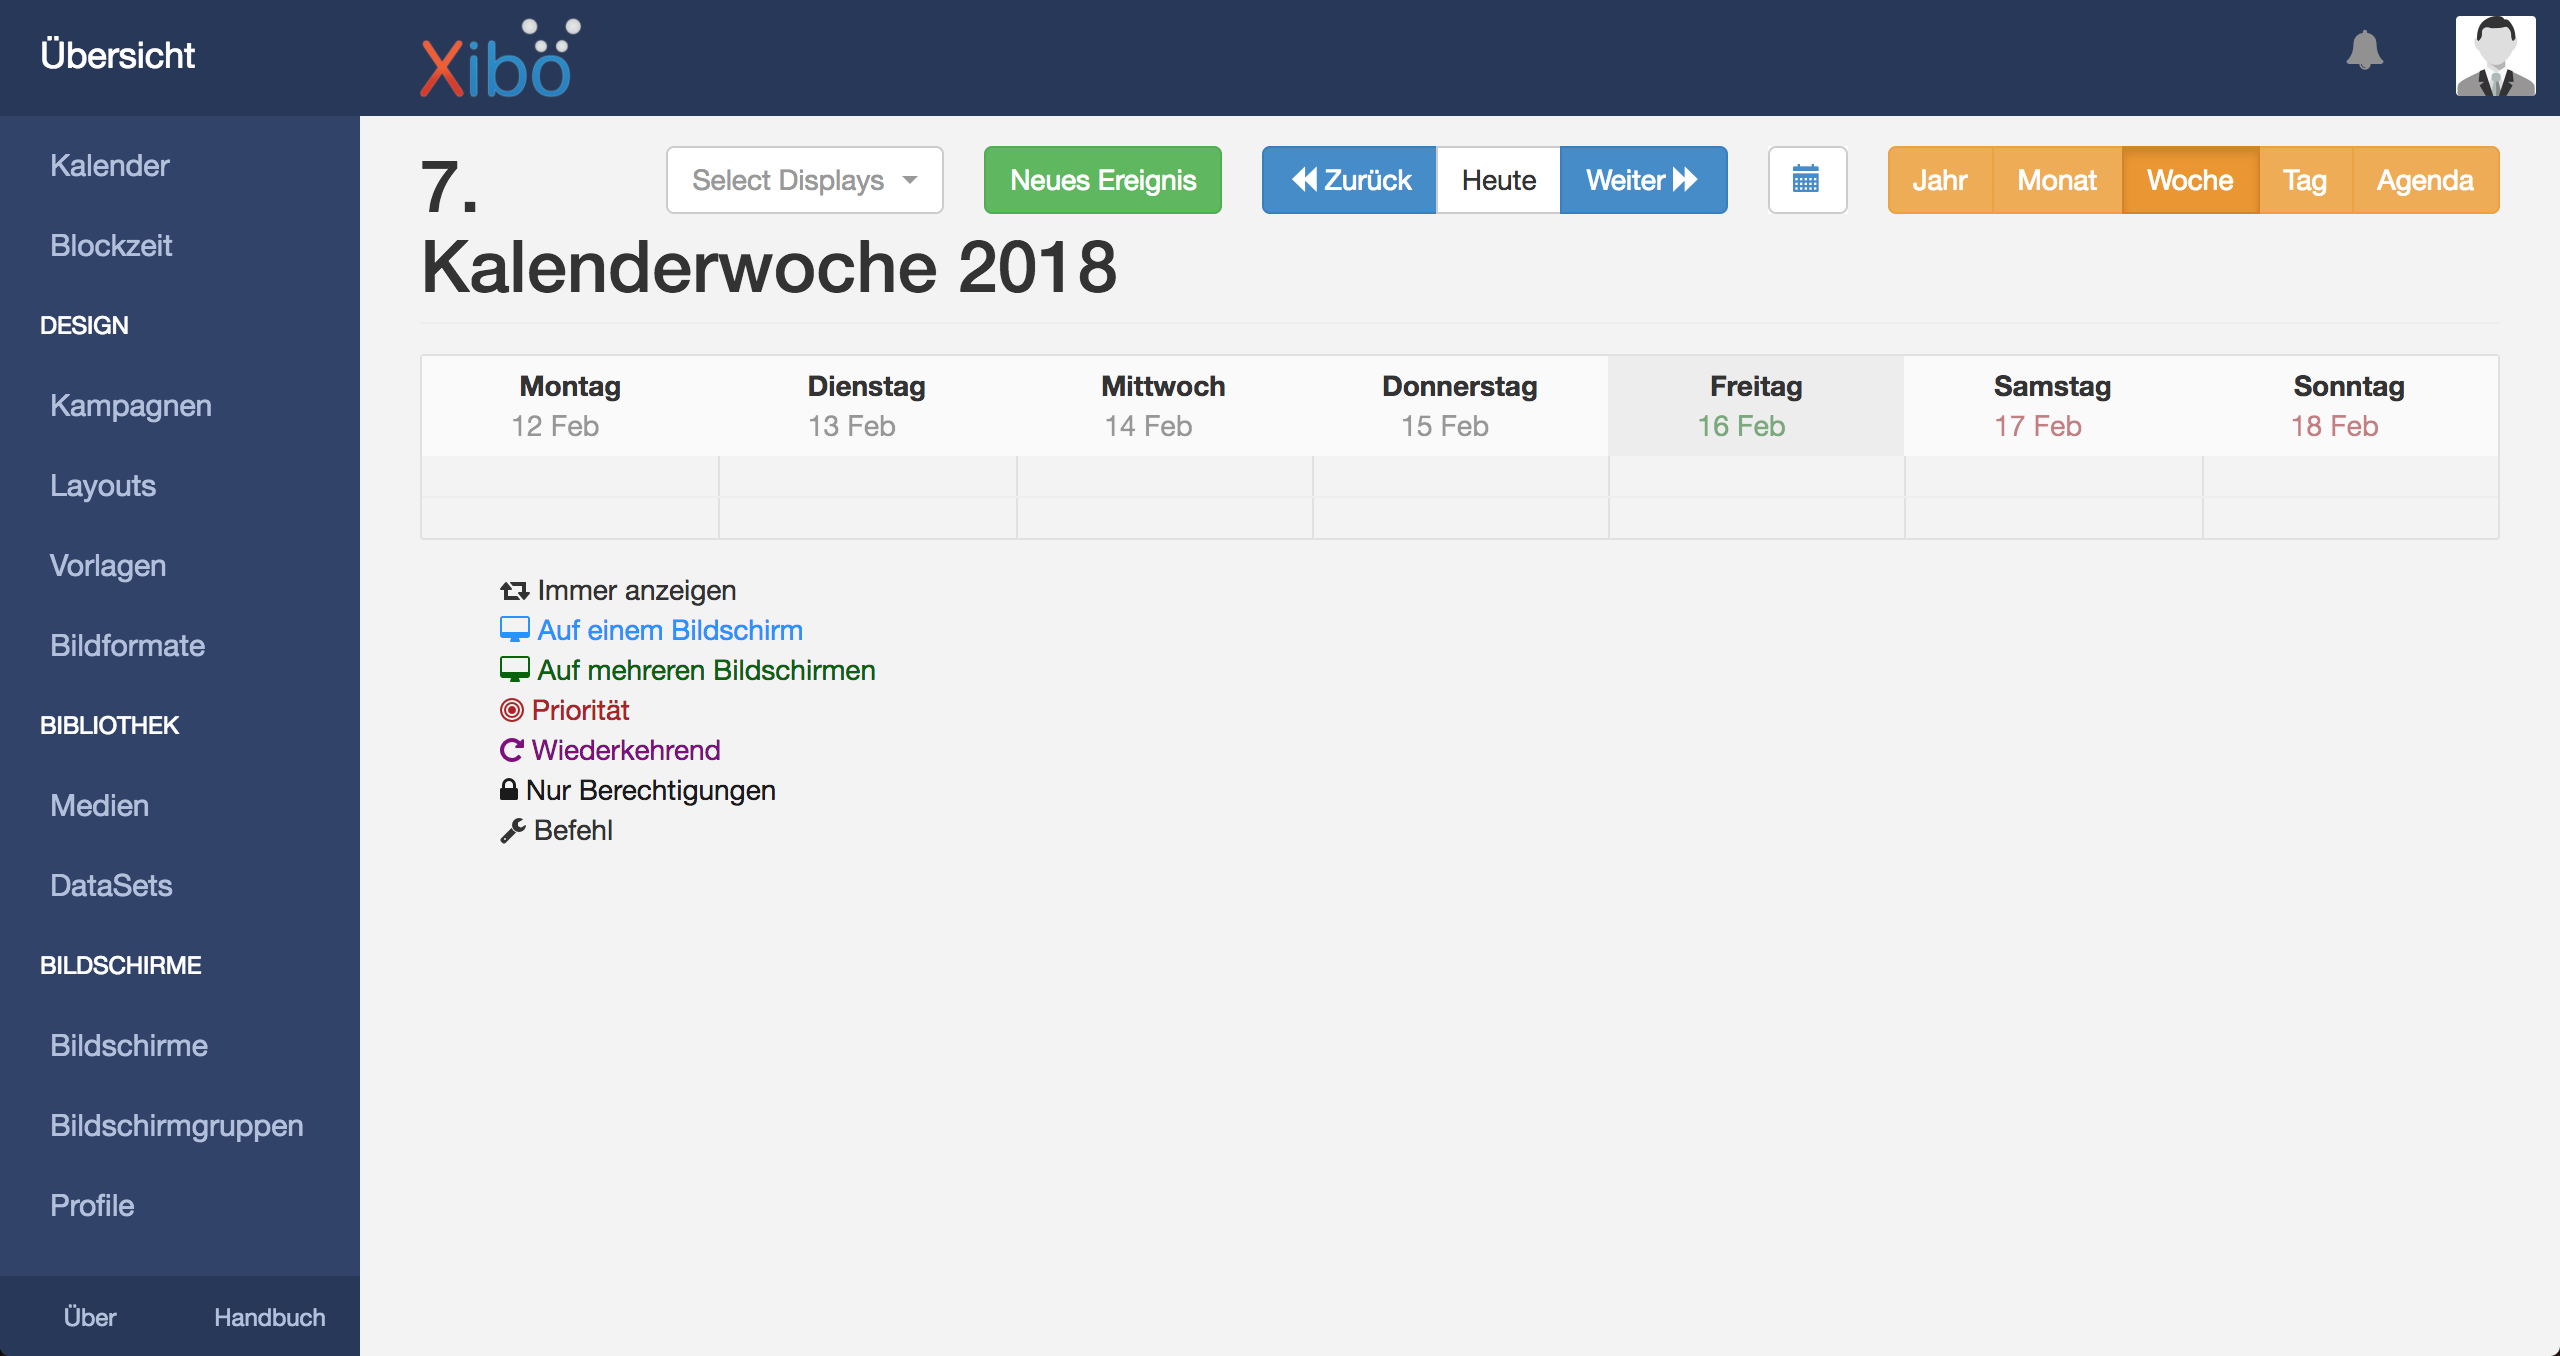
\includegraphics[width=1\textwidth]{images/xibo-basics-calendar}
  \label{Calendar}
\end{calendar}  
  
  \item {\em Layouts:} 
  Die Layout Funktion ist einer der wichtigsten Komponenten des Signage Systems es beschäftigt sich mit dem designen der Inhalte. Auf diese Funktion kommen wir noch einmal zurück
  
  \item {\em Bibliothek:} 
  Die Bibliothek Funktion ist zuständig für das Verwalten der Medien. Hier können Sie verschiedene Dateien hochladen.  Diese Medien können dann in Layouts eingebunden und angezeigt werden.
  
  \item {\em Benutzer:} 
  Im Menüpunkt Benutzer können neue Benutzer angelegt werden und bereits bestehende bearbeitet oder gelöscht werden. Dabei gibt es auch ein Rechte-System. Es könne auch Datenmengen Begrenzungen pro Benutzer eingestellt werden.
  
  \item {\em Einstellungen:} 
  Der Menöpunkt Einstellung gibt dem Nutzer die Möglichkeit verschiedene Optionen einzustellen. So sind zum Beispiel die richtige Zeitzone, E-Mail Benachrichtigungen wichtige Einstellungen die für ein Einwandfreies funktionieren des Xibo-Servers zuständig wichtig sind.
\end{enumerate}
 
\section{Designen mit XIBO}\label{sec:designexibo}
Beim Designen von einem neuen Layout im XIBO muss zuerst die Bildschirm auflösung ausgewählt werden. Und dem Layout ein passender Name zugewiesen werden sowie optional auch eine Beschreibung. 
 
\textbf{Layout Maske}
 
\begin{calendar}
  \centering
1 file change in working directory
View change
commit:c95ae5
WIP on master: Auto stash before merge of "master" and "origin/master"
